\item \textbf{Finally, repeat the analysis in 3 but for a VAR-based approach. Explore the relationships between the chosen variables using appropriate tools. Again, there is no fixed number of variables assigned – use your judgement and justify your decisions.  Using a VAR framework, show the impact of including additional variables in your prediction. Repeat the analysis in 2 (a) and (b) using the updated models.} 

\textit{Likewise the last question, we visualized the first nine signals to see what kind of data we have.} 

\begin{figure}[H]
    \centering
    \begin{minipage}[b]{1\textwidth}
        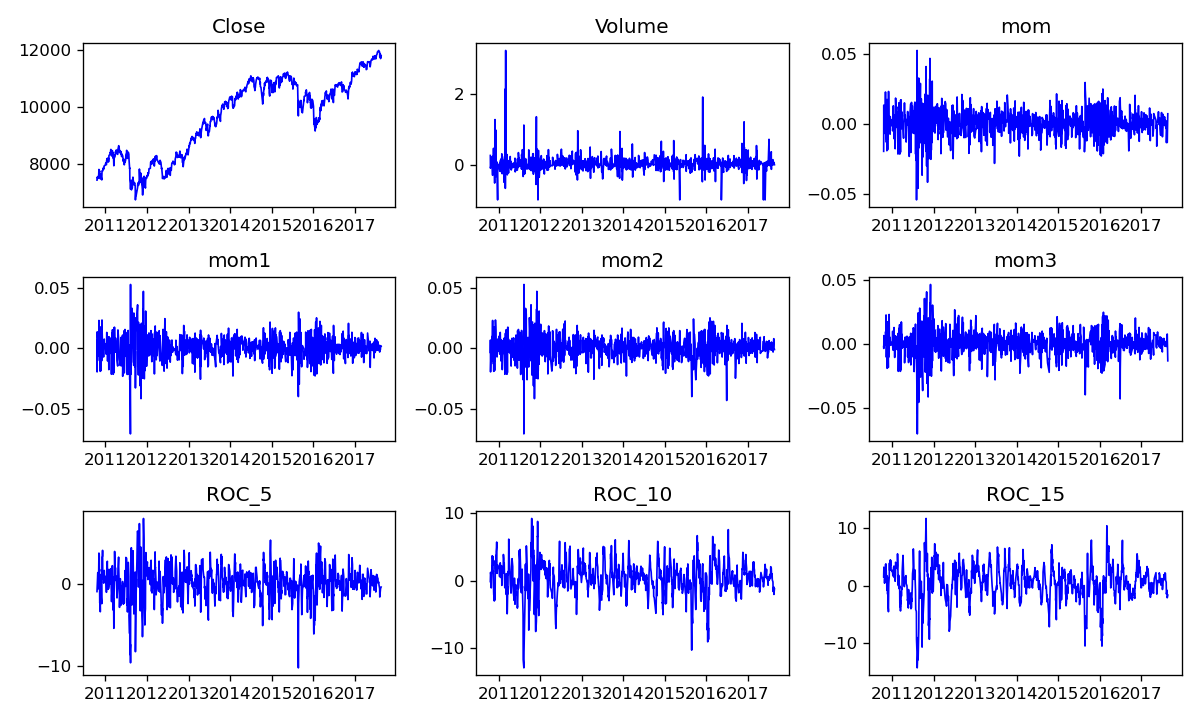
\includegraphics[width=\textwidth]{figures/Ass2/Ass2_Q3_raw_signal.png}
    \end{minipage}
    \caption{The visualization of the first nine columns.}
    \label{fig:Ass2_Q4_raw_signal}
\end{figure}




\textit{As these signals had the different range, we  standardized all data to have the same range. Figure \ref{fig:Ass2_Q4_standard_data} indicates the standardized signals. Also, we applied \gls{ADF} on these signals to find out that these signals were stationary or non-stationary. Table \ref{tab:Ass2_Q4_ADF_results} shows the result of this test on the dataset.}

\begin{figure}[H]
    \centering
    \begin{minipage}[b]{1\textwidth}
        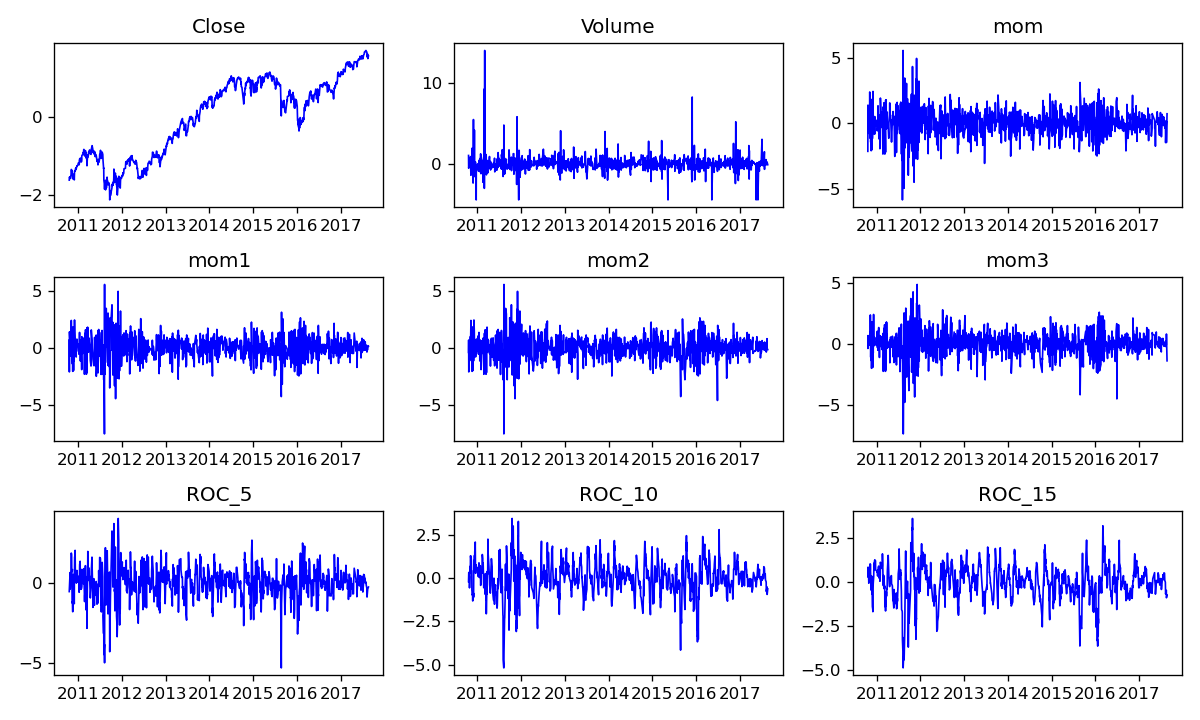
\includegraphics[width=\textwidth]{figures/Ass2/Ass2_Q4_standard_data.png}
    \end{minipage}
    \caption{The visualization of the first nine columns. Columns were standardized.}
    \label{fig:Ass2_Q4_standard_data}
\end{figure}


\begin{table}[H]
\centering
\caption{The result of the \gls{ADF} on the dataset.}
\label{tab:Ass2_Q4_ADF_results}
{\scriptsize
\begin{tabular}{lrrrrrrrrr}
\toprule
{} &        Close &        Volume &           mom &         mom1 &          mom2 &         mom3 &         ROC\_5 &        ROC\_10 &        ROC\_15 \\
\midrule
ADF Statistic               &    -1.08 & -14.88 & -12.13 &   -38.46 & -8.14 &   -20.97 & -10.61 & -9.75 & -6.99 \\
p-value                     &     0.720 &  1.5e-27 &  1.7e-22 &     0.00 &  9.8e-13 &     0.00 &  5.5e-19 &  7.9e-17 &  7.5e-10 \\
\#Lags Used                  &     2 &  4 &  11 &     0 &  20 &     2 &  9 &  6 &  16 \\
Number of Obs Used &  1111 &  1109 &  1102 &  1113 &  1093 &  1111 &  1104 &  1107 &  1097 \\
Critical Value (1\%)         &    -3.436 & -3.436 & -3.436 &    -3.436 & -3.436 &    -3.436 & -3.436 & -3.436 & -3.436 \\
Critical Value (5\%)         &    -2.864 & -2.864 & -2.864 &    -2.864 & -2.864 &    -2.864 & -2.864 & -2.864 & -2.864 \\
Critical Value (10\%)        &    -2.568 & -2.568 & -2.568 &    -2.568 & -2.568 &    -2.568 & -2.568 & -2.568 & -2.568 \\
\bottomrule
\end{tabular}
}
\end{table}

\textit{According to table \ref{tab:Ass2_Q4_ADF_results} all columns were stationary except the "Close price".  
We used a first-order differencing to turn this time series to a stationary data. Figures \ref{fig:Ass2_Q4_1diff_Close_signal} and \ref{fig:Ass2_Q4_PACF_ACF_1diff} indicate this $1^{st}$ order differencing signal along with its \gls{ACF} and \gls{PACF} plots. These two plots also show that the data got stationary.}

\begin{figure}[H]
    \centering
    \begin{minipage}[b]{1\textwidth}
        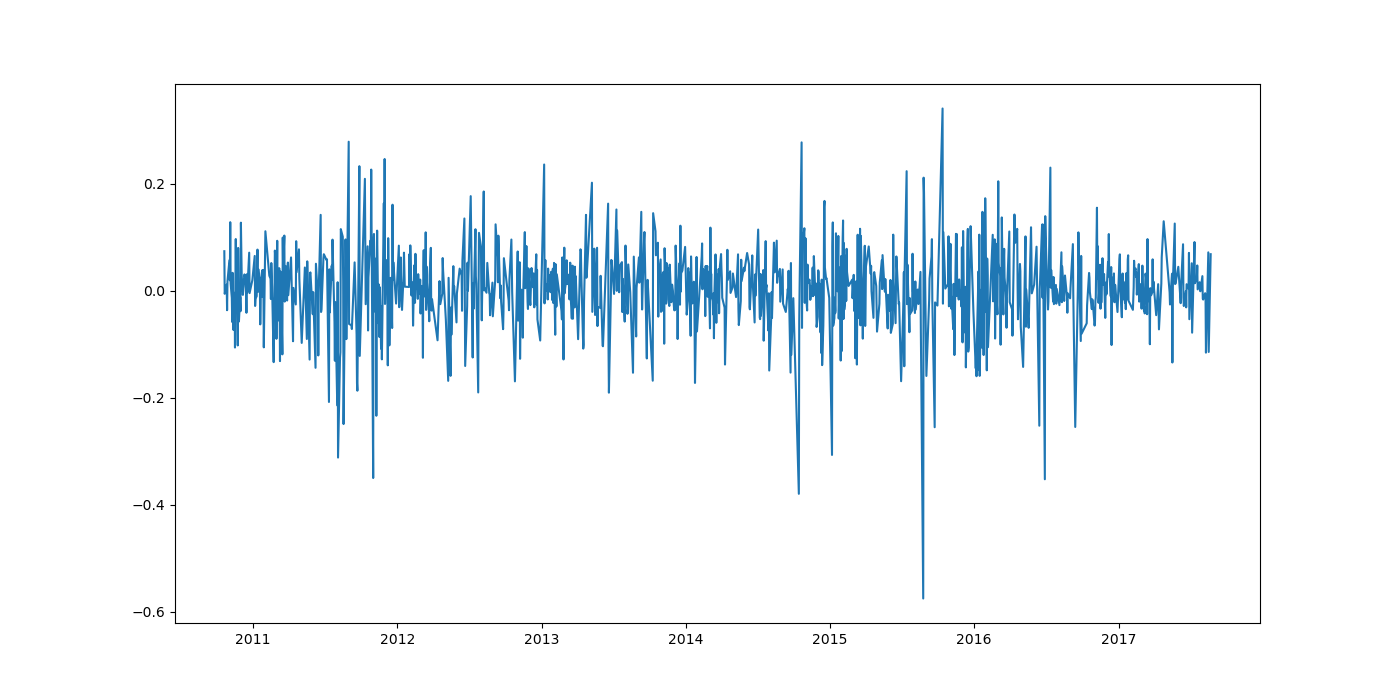
\includegraphics[width=\textwidth]{figures/Ass2/Ass2_Q4_1diff_Close_signal.png}
    \end{minipage}
    \caption{The $1^{st}$ order differencing of "Close price" data.}
    \label{fig:Ass2_Q4_1diff_Close_signal}
\end{figure}

\begin{figure}[H]
    \centering
    \begin{minipage}[b]{1\textwidth}
        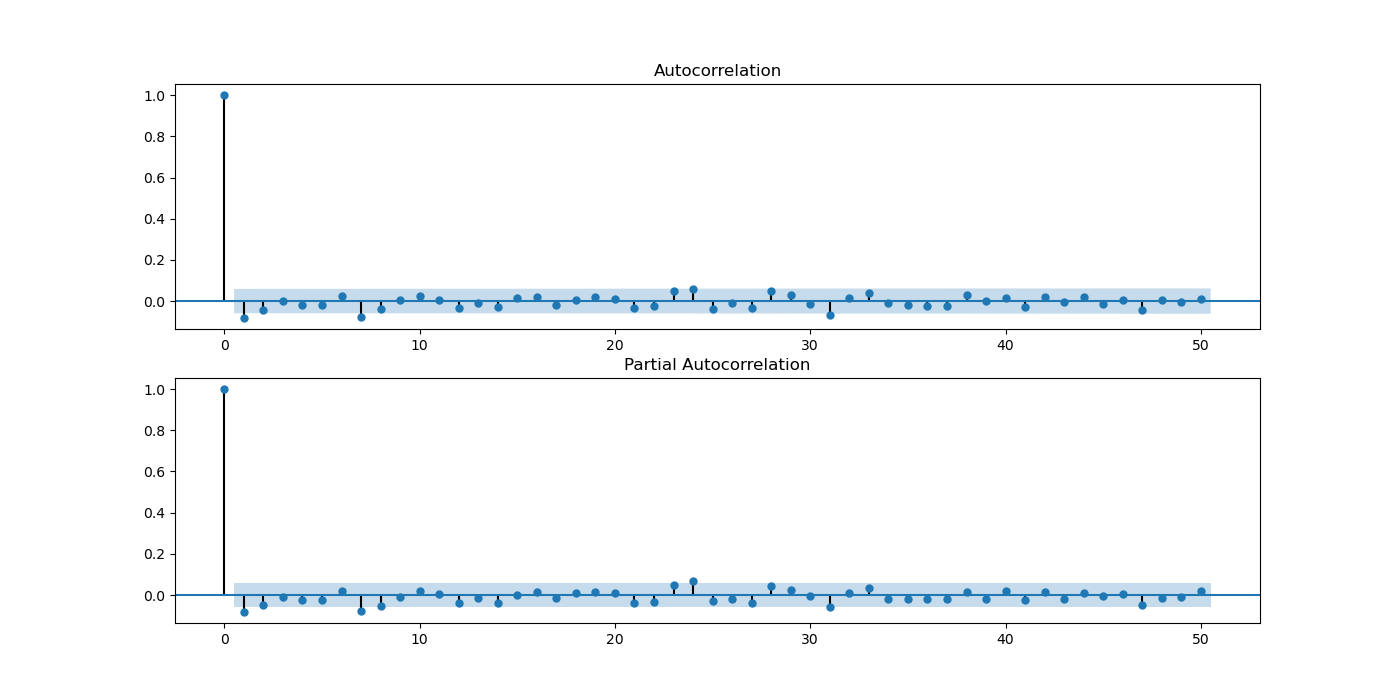
\includegraphics[width=\textwidth]{figures/Ass2/Ass2_Q3_PACF_ACF_1diff.png}
    \end{minipage}
    \caption{A plot of \gls{ACF} and \gls{PACF} on the $1^{st}$ order differencing in "Close price".}
    \label{fig:Ass2_Q4_PACF_ACF_1diff}
\end{figure}

\textit{After transforming and making stationary, we applied 
\gls{ACF} and \gls{PACF} on the our target variable, here it was "Close price". Since PACF (see figure \ref{fig:Ass2_Q4_PACF_ACF_1diff}) had one significant lag, it can conclude that order of AR was one.}

\textit{Also to find the best fitted model, we searched on different orders. For searching area, we used all lags between 1 and 13. Figure \ref{fig:Ass2_Q4_AIC_plot} shows the \gls{AIC} over the different orders. The best order in terms of simplicity and goodness belonged to order 7 (VAR(7) model). }

\begin{figure}[H]
    \centering
    \begin{minipage}[b]{1\textwidth}
        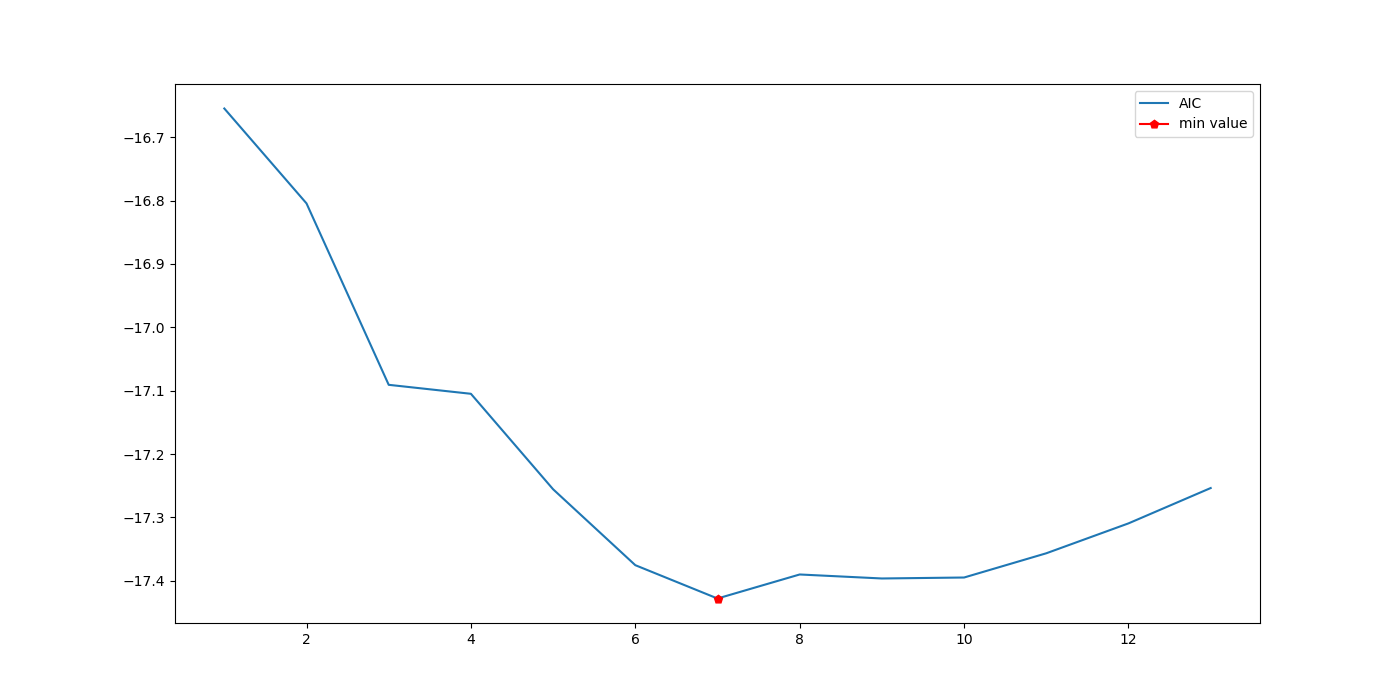
\includegraphics[width=\textwidth]{manuscript/src/figures/Ass2/Ass2_Q4_AIC_plot.png}
    \end{minipage}
    \caption{The \gls{AIC} over the different orders of VAR model.}
    \label{fig:Ass2_Q4_AIC_plot}
\end{figure}

\textit{Figure \ref{fig:Ass2_Q4_residual_plot} indicates the residual of fitted model only for the first variable. As this plot illustrates, the residual signal of model had a Gaussian distribution with zero mean. In addition, the \gls{ACF} plot shows that this signal is a stationary signal.}



\begin{figure}[H]
    \centering
    \begin{minipage}[b]{1\textwidth}
        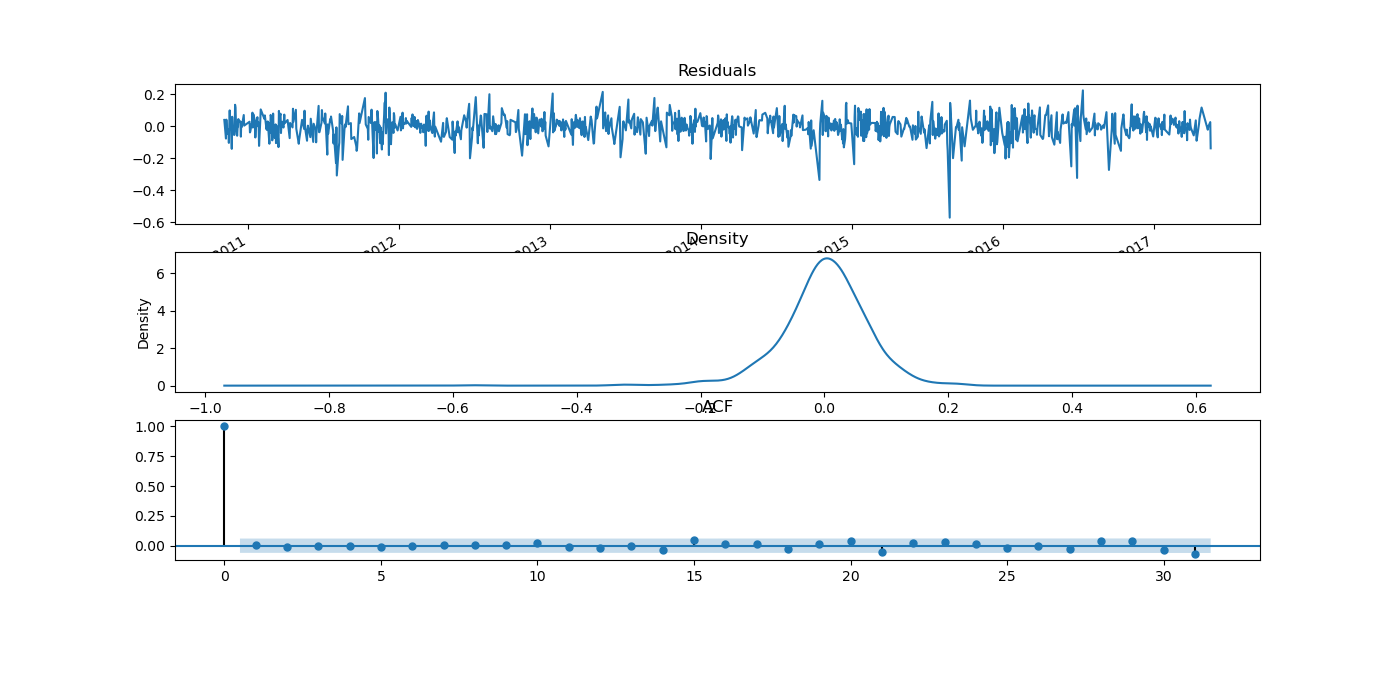
\includegraphics[width=\textwidth]{manuscript/src/figures/Ass2/Ass2_Q4_residual_plot.png}
    \end{minipage}
    \caption{The residual of the fitted model.}
    \label{fig:Ass2_Q4_residual_plot}
\end{figure}


\textit{In addition, we applied Durbin Watson Statistic to estimate their correlation between residuals. This correlation shows whether or not pattern has any leftover pattern in the residuals. As table \ref{tab:Ass2_Q4_DW_results} indicates Durbin Watson results were close to 2. It means there are not correlation between residuals. } 

\begin{table}[H]
\centering
\caption{The result of Durbin Watson test on the dataset.}
\label{tab:Ass2_Q4_DW_results}
\begin{tabular}{rll}
\toprule
\# &  Variable Name &   The result \\
\midrule
1 & Close   &   1.99\\
2 & mom     &   1.98\\
3 & mom1    &   2.0\\
4 & ROC\_5   &   1.99\\
5 & ROC\_10  &   1.99\\
6 & ROC\_15  &   1.97\\
7 & ROC\_20  &   1.97\\
8 & EMA\_10  &   2.0\\
9 & EMA\_20  &   2.0\\
10 & EMA\_50  &   2.0\\
11 & EMA\_200 &        2.0\\
12 & Oil     &    2.0\\
\bottomrule
\end{tabular}




\end{table}




\textit{Figure \ref{fig:Ass2_Q4_residual_plot} indicates the residual of fitted model only for the first variable. As this plot illustrates, the residual signal of model had a Gaussian distribution with zero mean. In addition, the \gls{ACF} plot shows that this signal is a stationary signal.}



\begin{figure}[H]
    \centering
    \begin{minipage}[b]{1\textwidth}
        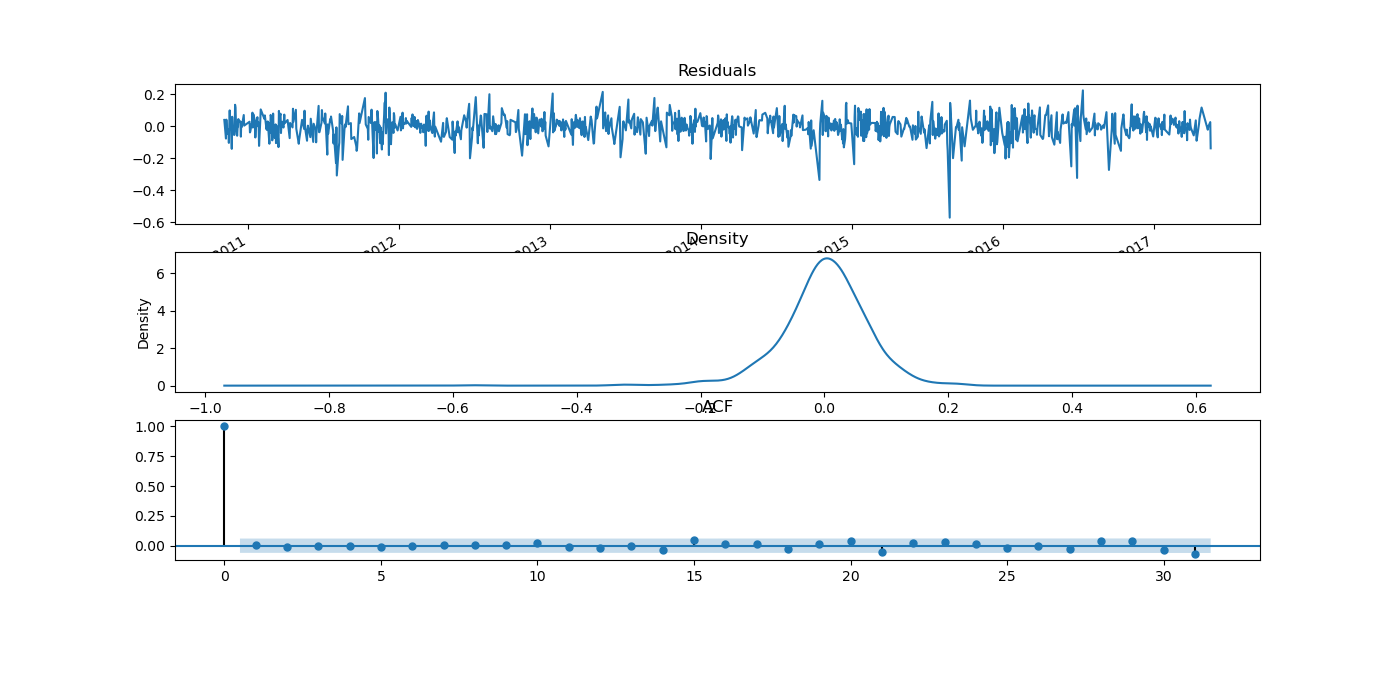
\includegraphics[width=\textwidth]{manuscript/src/figures/Ass2/Ass2_Q4_residual_plot.png}
    \end{minipage}
    \caption{The residual of the fitted model.}
    \label{fig:Ass2_Q4_residual_plot}
\end{figure}

\textit{To forecast, we split data into test and train set like last two parts. After prediction, we reversed differencing and standardization to get the real forecast. Figures \ref{fig:Ass2_Q4_Forecast_vs_Actuals} and \ref{fig:Ass2_Q4_Forecast_vs_Actuals_of_close} demonstrate the output of the fitted model. As can be seen, the model could predict like the \gls{arima} (question 2a), and because of using the exogenous variables, the prediction had some ripples that followed the the actual data. These ripples decreased the RMS error to 271.592.} 

\begin{figure}[H]
    \centering
    \begin{minipage}[b]{1\textwidth}
        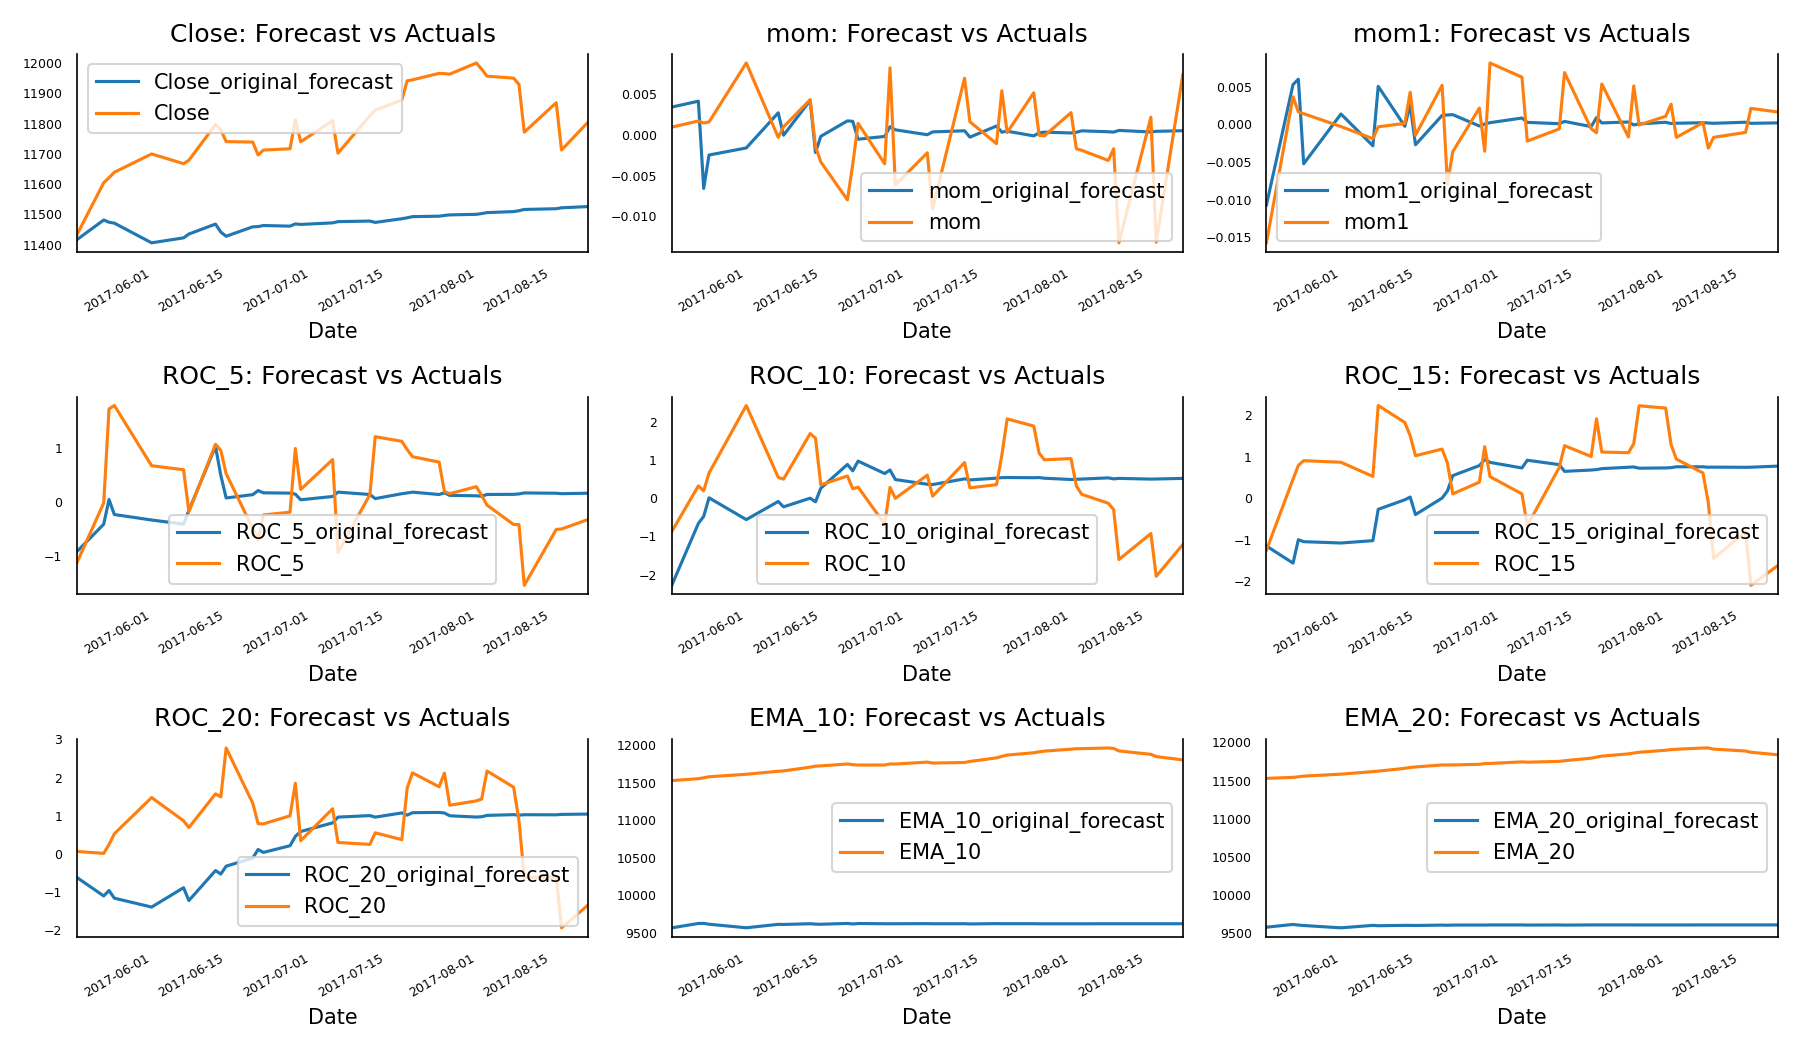
\includegraphics[width=\textwidth]{manuscript/src/figures/Ass2/Ass2_Q4_Forecast_vs_Actuals.png}
    \end{minipage}
    \caption{The prediction and actual data of VAR model.}
    \label{fig:Ass2_Q4_Forecast_vs_Actuals}
\end{figure}

\begin{figure}[H]
    \centering
    \begin{minipage}[b]{1\textwidth}
        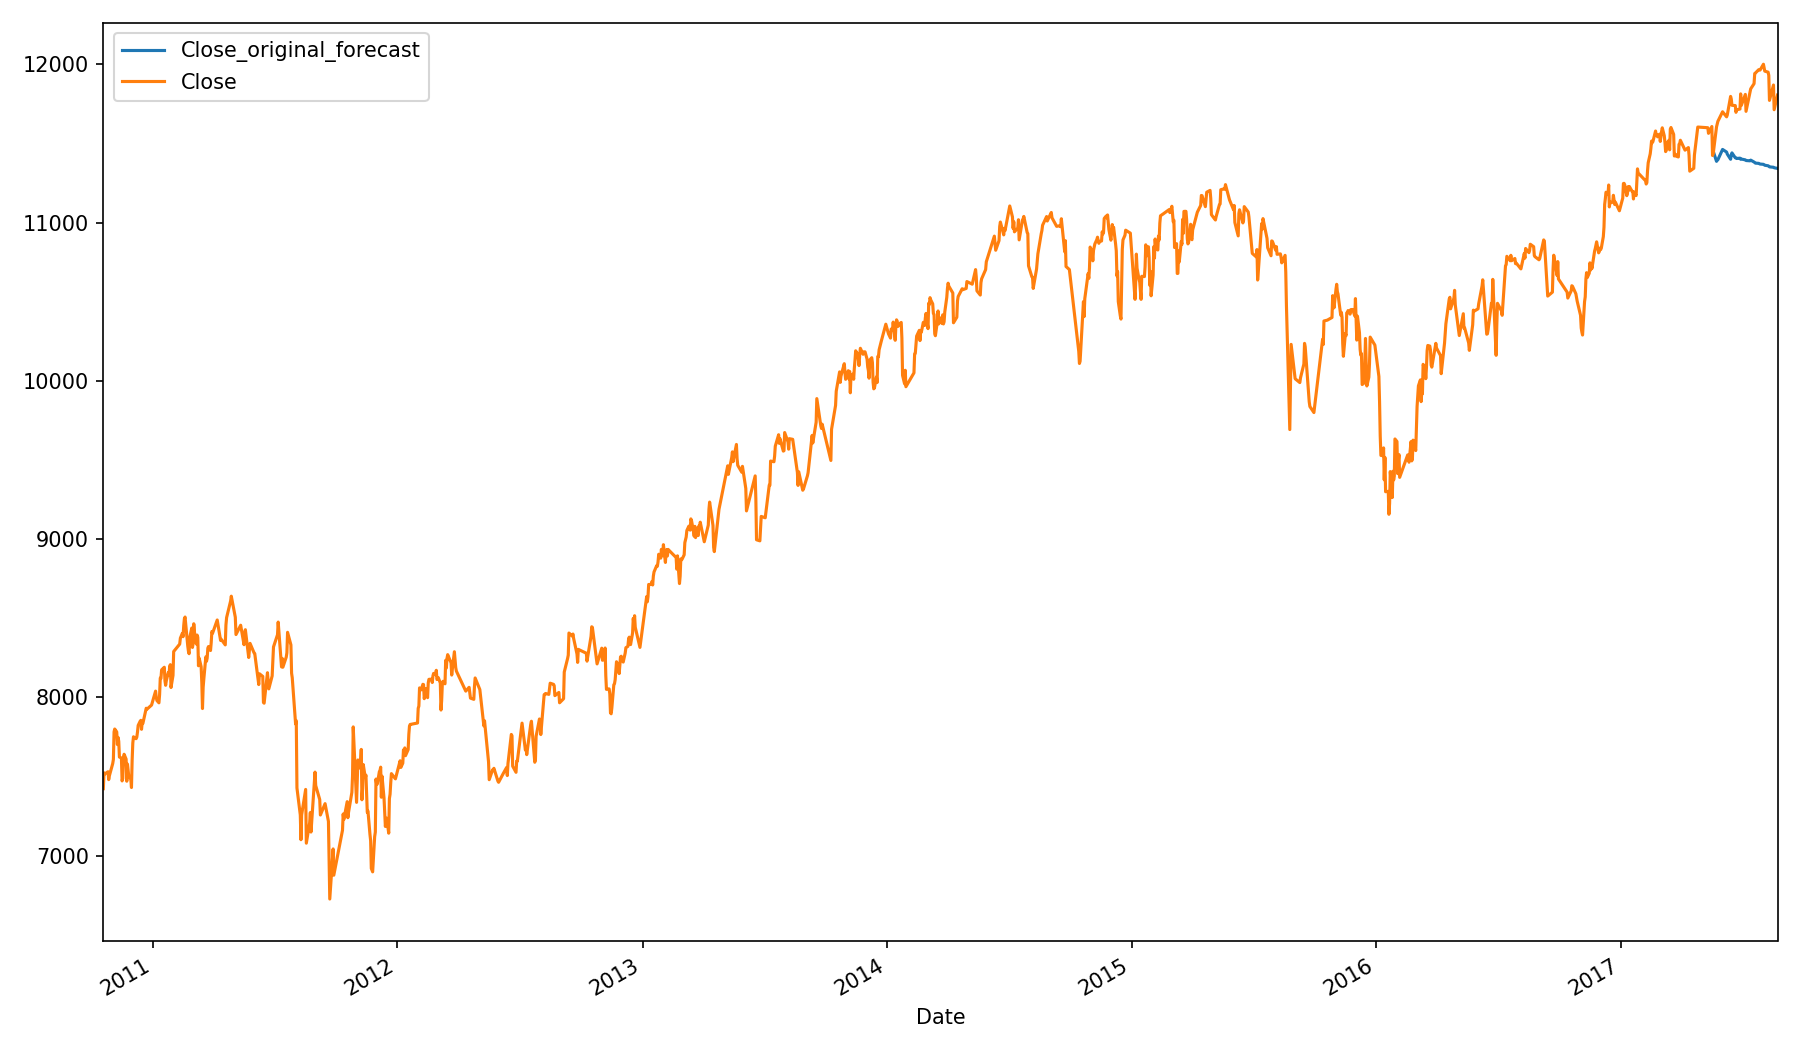
\includegraphics[width=\textwidth]{manuscript/src/figures/Ass2/Ass2_Q4_Forecast_vs_Actuals_of_close.png}
    \end{minipage}
    \caption{The prediction and actual data of VAR model.}
    \label{fig:Ass2_Q4_Forecast_vs_Actuals_of_close}
\end{figure}




\textit{For the rolling window approach, we used the same procedure in question 2. Figures \ref{fig:Ass2_Q4_Rolling_Forecast_vs_Actuals} and \ref{fig:Ass2_Q4_Rolling_Forecast_vs_Actuals_of_close} demonstrate the output of the rolling window model for VAR. As can be seen, the model could follow the the test set better than previous models. The RMS error decreased to 261.581. Since we used additional information of exogenous variables, the prediction had some ripples.}

\begin{figure}[H]
    \centering
    \begin{minipage}[b]{1\textwidth}
        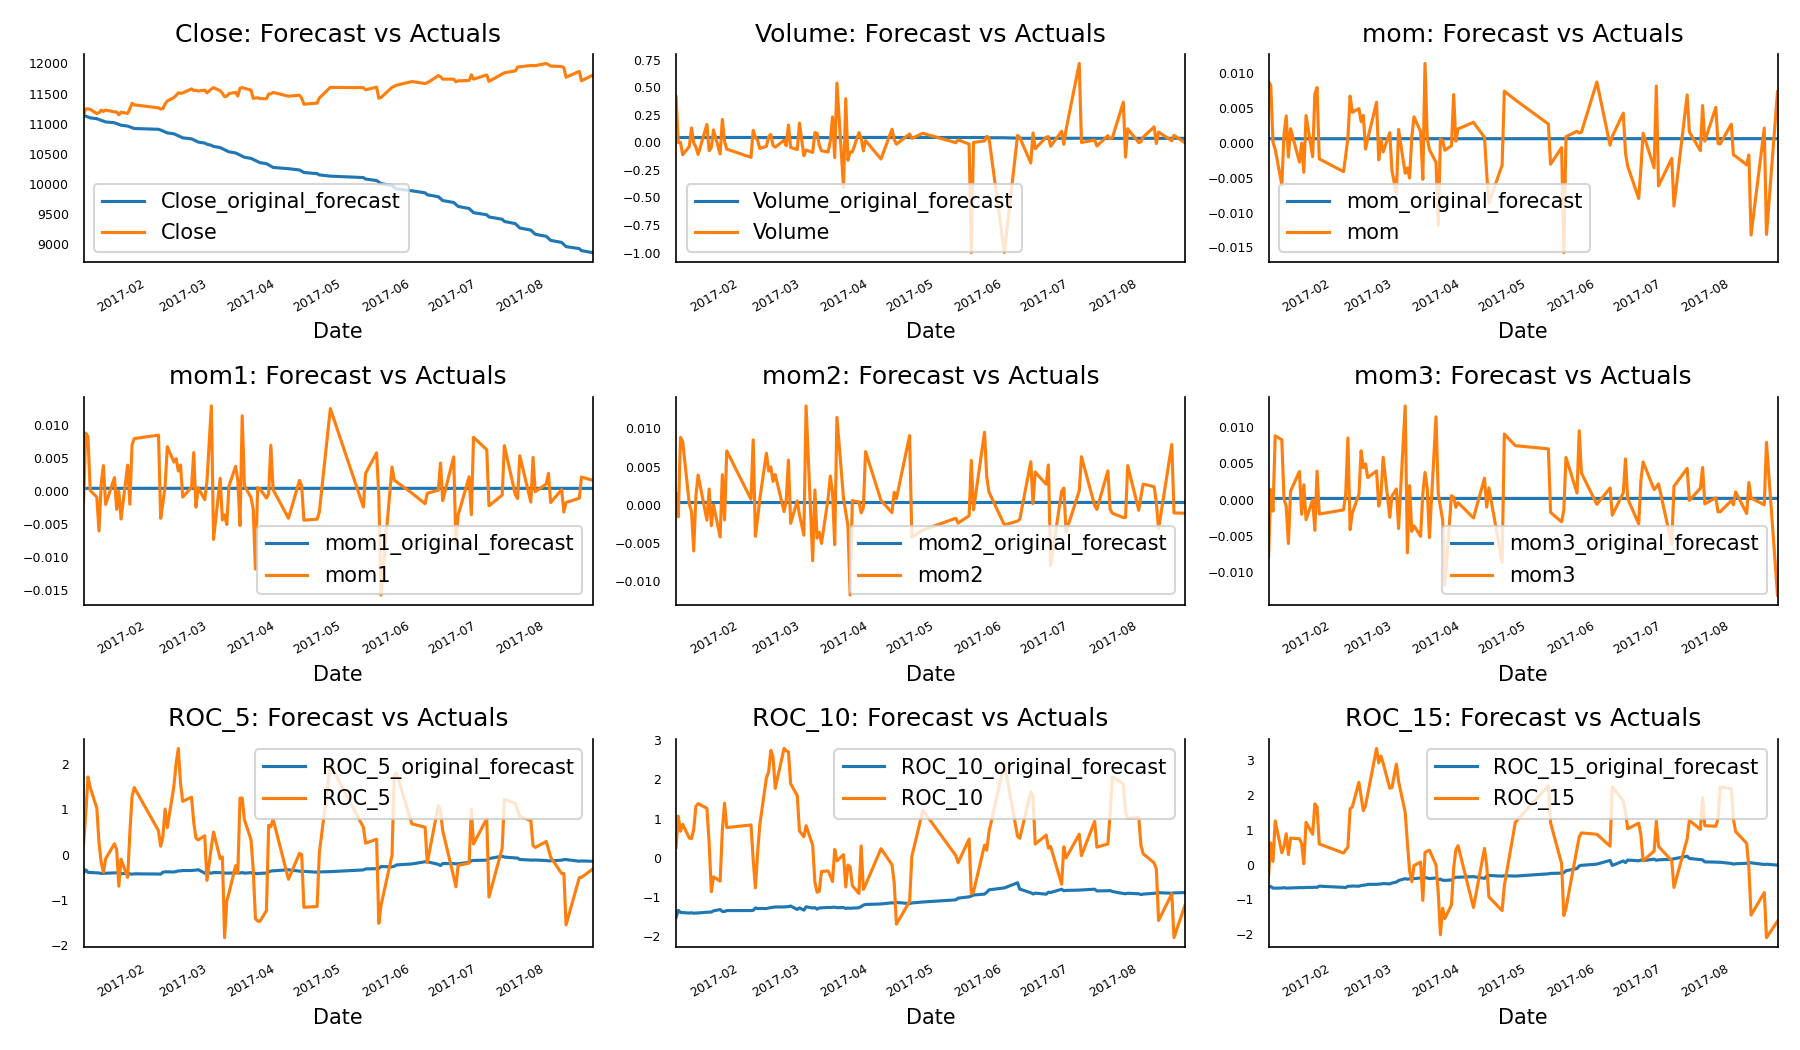
\includegraphics[width=\textwidth]{manuscript/src/figures/Ass2/Ass2_Q4_Rolling_Forecast_vs_Actuals.png}
    \end{minipage}
    \caption{The prediction and actual data of VAR model.}
    \label{fig:Ass2_Q4_Rolling_Forecast_vs_Actuals}
\end{figure}

\begin{figure}[H]
    \centering
    \begin{minipage}[b]{1\textwidth}
        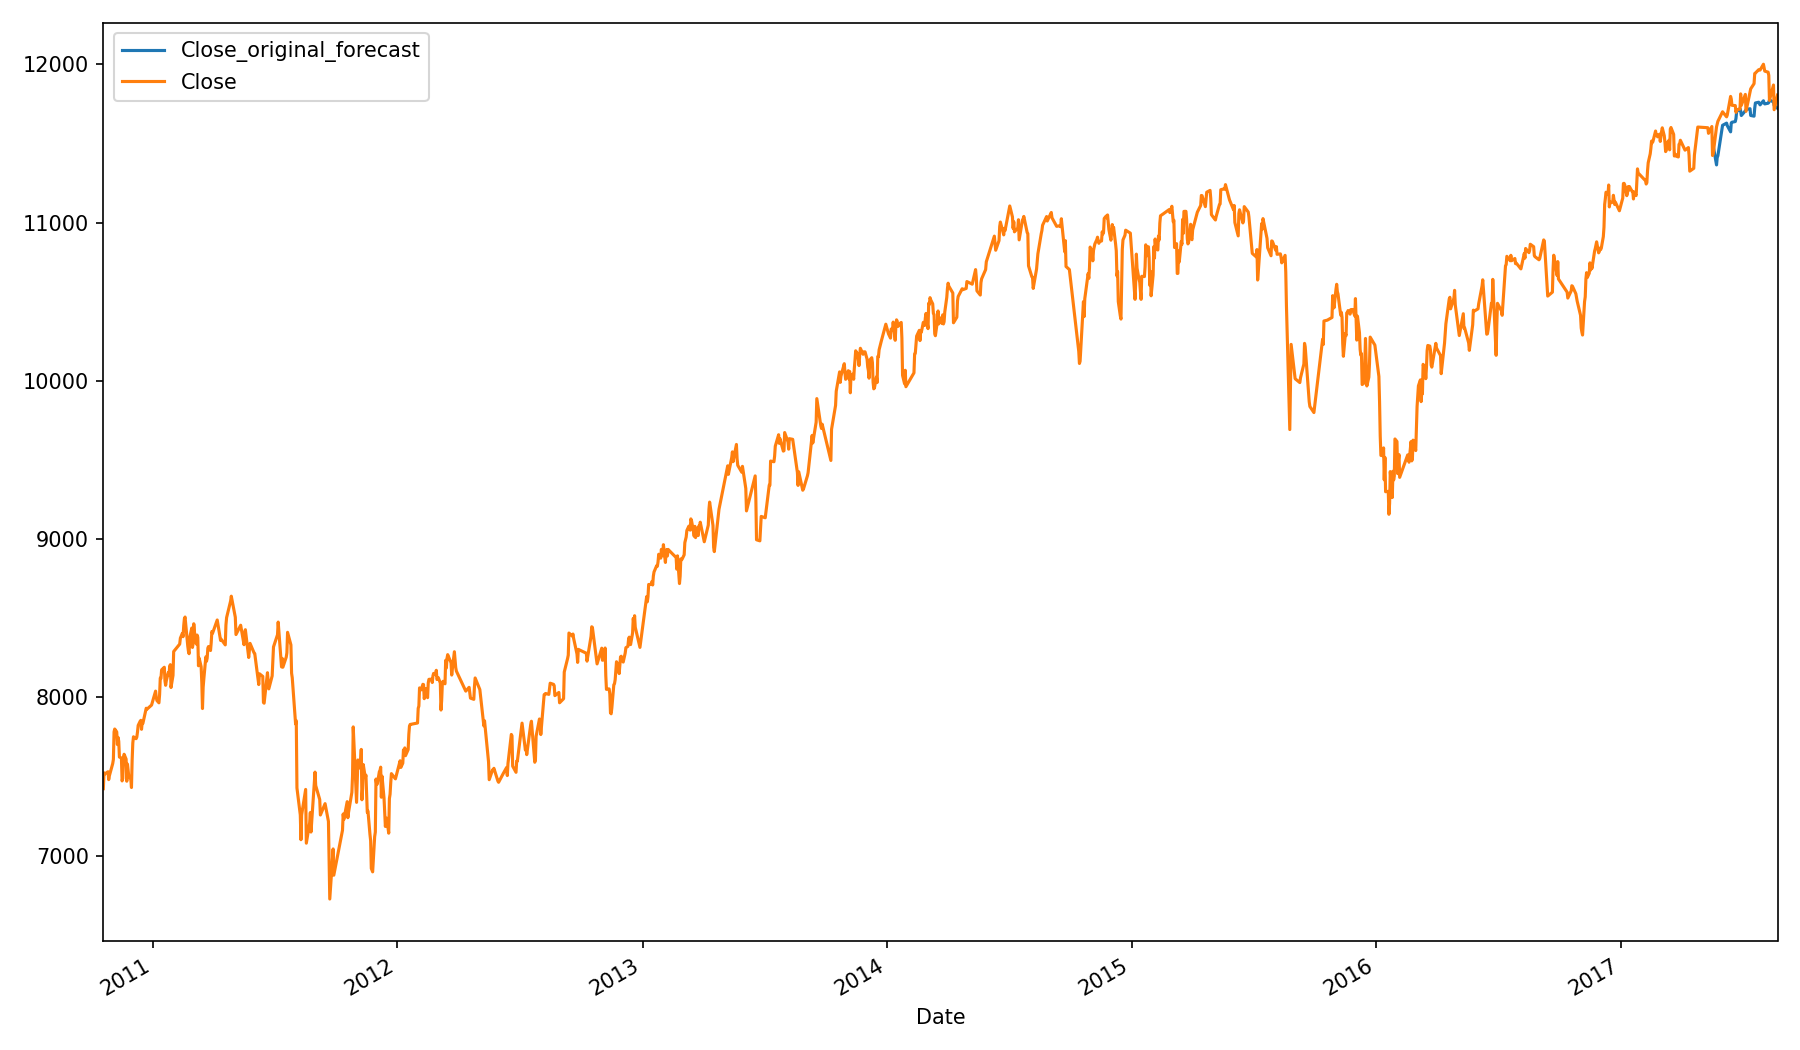
\includegraphics[width=\textwidth]{manuscript/src/figures/Ass2/Ass2_Q4_Rolling_Forecast_vs_Actuals_of_close.png}
    \end{minipage}
    \caption{The prediction and actual data of VAR model.}
    \label{fig:Ass2_Q4_Rolling_Forecast_vs_Actuals_of_close}
\end{figure}